
As explained before, we use the \verb|diff| utility to compare two SAM output files. Having the number of different lines between two files, we can calculate a percentage of difference. To be able to compare the outputs, they must be in the same order: this is why we have to run the program on single thread for this verification. We measure the influence of the seed-only paradigm on the results. It is worth noting that, in addition to the best alignment with its score, BWA outputs alternative alignments which may lead to different, lower quality results. In the case of seed-only paradigm, it regularly happens that the main result is matching, yet the secondary alignments present very slight differences. Since these values are rarely useful in real use cases, we also compared the outputs without these results, to know the difference only for the final alignment. We implemented a "seed-only" version of BWA to control that our kernel implementation on GPU is correct. The results are presented on figure~\ref{fig:result-diff-srr150}.

\begin{figure}[h!]
	\centering
	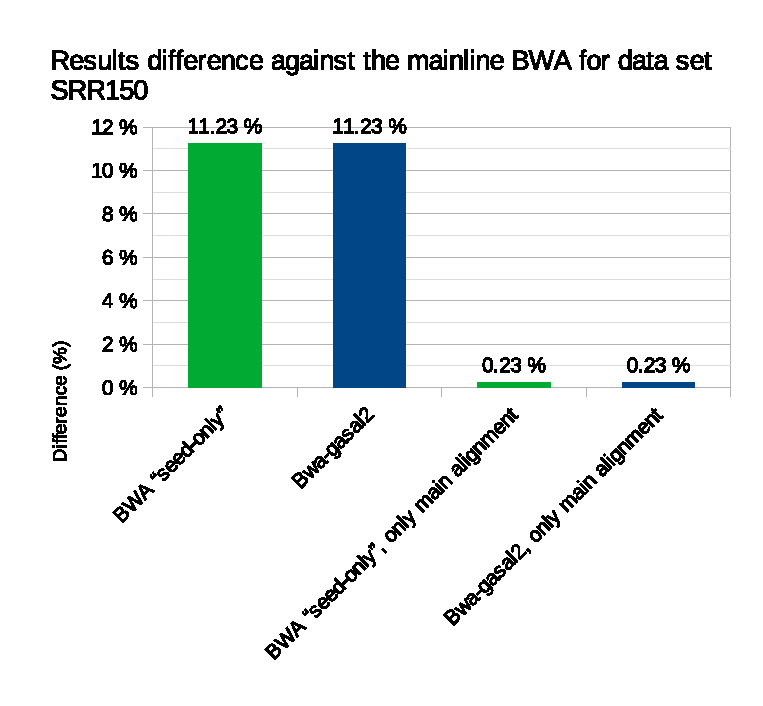
\includegraphics[width=1\linewidth]{srr150/result-diff-srr150}
	\caption{Difference in the result with the mainline version of BWA}
	\label{fig:result-diff-srr150}
\end{figure}

First, we checked that the results between the seed-only version of BWA and our bwa-gasal2 have the same output. They present the same number of difference with the mainline program, and have the same content.

We notice that the seed-only paradigm globally introduces a noticeable number of differences. 11.23\% of the lines are not matching. Still, when we set aside the secondary results, this percentage drops to a mere 0.23\%. This is small enough to consider it acceptable.


